% Options for packages loaded elsewhere
\PassOptionsToPackage{unicode}{hyperref}
\PassOptionsToPackage{hyphens}{url}
\PassOptionsToPackage{dvipsnames,svgnames,x11names}{xcolor}
%
\documentclass[
]{article}
\title{Assignment 2}
\author{Nguyen Xuan Binh}
\date{}

\usepackage{amsmath,amssymb}
\usepackage{lmodern}
\usepackage{iftex}
\ifPDFTeX
  \usepackage[T1]{fontenc}
  \usepackage[utf8]{inputenc}
  \usepackage{textcomp} % provide euro and other symbols
\else % if luatex or xetex
  \usepackage{unicode-math}
  \defaultfontfeatures{Scale=MatchLowercase}
  \defaultfontfeatures[\rmfamily]{Ligatures=TeX,Scale=1}
\fi
% Use upquote if available, for straight quotes in verbatim environments
\IfFileExists{upquote.sty}{\usepackage{upquote}}{}
\IfFileExists{microtype.sty}{% use microtype if available
  \usepackage[]{microtype}
  \UseMicrotypeSet[protrusion]{basicmath} % disable protrusion for tt fonts
}{}
\makeatletter
\@ifundefined{KOMAClassName}{% if non-KOMA class
  \IfFileExists{parskip.sty}{%
    \usepackage{parskip}
  }{% else
    \setlength{\parindent}{0pt}
    \setlength{\parskip}{6pt plus 2pt minus 1pt}}
}{% if KOMA class
  \KOMAoptions{parskip=half}}
\makeatother
\usepackage{xcolor}
\IfFileExists{xurl.sty}{\usepackage{xurl}}{} % add URL line breaks if available
\IfFileExists{bookmark.sty}{\usepackage{bookmark}}{\usepackage{hyperref}}
\hypersetup{
  pdftitle={Assignment 2},
  pdfauthor={Nguyen Xuan Binh},
  colorlinks=true,
  linkcolor={Maroon},
  filecolor={Maroon},
  citecolor={Blue},
  urlcolor={blue},
  pdfcreator={LaTeX via pandoc}}
\urlstyle{same} % disable monospaced font for URLs
\usepackage[margin=1in]{geometry}
\usepackage{color}
\usepackage{fancyvrb}
\newcommand{\VerbBar}{|}
\newcommand{\VERB}{\Verb[commandchars=\\\{\}]}
\DefineVerbatimEnvironment{Highlighting}{Verbatim}{commandchars=\\\{\}}
% Add ',fontsize=\small' for more characters per line
\usepackage{framed}
\definecolor{shadecolor}{RGB}{248,248,248}
\newenvironment{Shaded}{\begin{snugshade}}{\end{snugshade}}
\newcommand{\AlertTok}[1]{\textcolor[rgb]{0.94,0.16,0.16}{#1}}
\newcommand{\AnnotationTok}[1]{\textcolor[rgb]{0.56,0.35,0.01}{\textbf{\textit{#1}}}}
\newcommand{\AttributeTok}[1]{\textcolor[rgb]{0.77,0.63,0.00}{#1}}
\newcommand{\BaseNTok}[1]{\textcolor[rgb]{0.00,0.00,0.81}{#1}}
\newcommand{\BuiltInTok}[1]{#1}
\newcommand{\CharTok}[1]{\textcolor[rgb]{0.31,0.60,0.02}{#1}}
\newcommand{\CommentTok}[1]{\textcolor[rgb]{0.56,0.35,0.01}{\textit{#1}}}
\newcommand{\CommentVarTok}[1]{\textcolor[rgb]{0.56,0.35,0.01}{\textbf{\textit{#1}}}}
\newcommand{\ConstantTok}[1]{\textcolor[rgb]{0.00,0.00,0.00}{#1}}
\newcommand{\ControlFlowTok}[1]{\textcolor[rgb]{0.13,0.29,0.53}{\textbf{#1}}}
\newcommand{\DataTypeTok}[1]{\textcolor[rgb]{0.13,0.29,0.53}{#1}}
\newcommand{\DecValTok}[1]{\textcolor[rgb]{0.00,0.00,0.81}{#1}}
\newcommand{\DocumentationTok}[1]{\textcolor[rgb]{0.56,0.35,0.01}{\textbf{\textit{#1}}}}
\newcommand{\ErrorTok}[1]{\textcolor[rgb]{0.64,0.00,0.00}{\textbf{#1}}}
\newcommand{\ExtensionTok}[1]{#1}
\newcommand{\FloatTok}[1]{\textcolor[rgb]{0.00,0.00,0.81}{#1}}
\newcommand{\FunctionTok}[1]{\textcolor[rgb]{0.00,0.00,0.00}{#1}}
\newcommand{\ImportTok}[1]{#1}
\newcommand{\InformationTok}[1]{\textcolor[rgb]{0.56,0.35,0.01}{\textbf{\textit{#1}}}}
\newcommand{\KeywordTok}[1]{\textcolor[rgb]{0.13,0.29,0.53}{\textbf{#1}}}
\newcommand{\NormalTok}[1]{#1}
\newcommand{\OperatorTok}[1]{\textcolor[rgb]{0.81,0.36,0.00}{\textbf{#1}}}
\newcommand{\OtherTok}[1]{\textcolor[rgb]{0.56,0.35,0.01}{#1}}
\newcommand{\PreprocessorTok}[1]{\textcolor[rgb]{0.56,0.35,0.01}{\textit{#1}}}
\newcommand{\RegionMarkerTok}[1]{#1}
\newcommand{\SpecialCharTok}[1]{\textcolor[rgb]{0.00,0.00,0.00}{#1}}
\newcommand{\SpecialStringTok}[1]{\textcolor[rgb]{0.31,0.60,0.02}{#1}}
\newcommand{\StringTok}[1]{\textcolor[rgb]{0.31,0.60,0.02}{#1}}
\newcommand{\VariableTok}[1]{\textcolor[rgb]{0.00,0.00,0.00}{#1}}
\newcommand{\VerbatimStringTok}[1]{\textcolor[rgb]{0.31,0.60,0.02}{#1}}
\newcommand{\WarningTok}[1]{\textcolor[rgb]{0.56,0.35,0.01}{\textbf{\textit{#1}}}}
\usepackage{graphicx}
\makeatletter
\def\maxwidth{\ifdim\Gin@nat@width>\linewidth\linewidth\else\Gin@nat@width\fi}
\def\maxheight{\ifdim\Gin@nat@height>\textheight\textheight\else\Gin@nat@height\fi}
\makeatother
% Scale images if necessary, so that they will not overflow the page
% margins by default, and it is still possible to overwrite the defaults
% using explicit options in \includegraphics[width, height, ...]{}
\setkeys{Gin}{width=\maxwidth,height=\maxheight,keepaspectratio}
% Set default figure placement to htbp
\makeatletter
\def\fps@figure{htbp}
\makeatother
\setlength{\emergencystretch}{3em} % prevent overfull lines
\providecommand{\tightlist}{%
  \setlength{\itemsep}{0pt}\setlength{\parskip}{0pt}}
\setcounter{secnumdepth}{-\maxdimen} % remove section numbering
\usepackage{amssymb}
\ifLuaTeX
  \usepackage{selnolig}  % disable illegal ligatures
\fi

\begin{document}
\maketitle

\hypertarget{homework-problem-1-pca-for-simulated-data}{%
\section{Homework Problem 1: PCA for Simulated
Data}\label{homework-problem-1-pca-for-simulated-data}}

Simulate 100 observations from bivariate normal distribution with
parameters:\\

\(\quad\quad\quad\quad\quad\quad\quad\quad\mu=\begin{pmatrix} 4\\7\end{pmatrix}, \quad \Sigma=\begin{pmatrix}10 & 6\\6 & 8\end{pmatrix}.\)

\hypertarget{a}{%
\subsection{a)}\label{a}}

Plot the data. Label the data points with the corresponding observation
number.

\begin{Shaded}
\begin{Highlighting}[]
\FunctionTok{library}\NormalTok{(}\StringTok{"ggplot2"}\NormalTok{)}
\end{Highlighting}
\end{Shaded}

\begin{verbatim}
## Warning: package 'ggplot2' was built under R version 4.1.3
\end{verbatim}

\begin{Shaded}
\begin{Highlighting}[]
\FunctionTok{library}\NormalTok{(}\StringTok{"mvtnorm"}\NormalTok{)}
\end{Highlighting}
\end{Shaded}

\begin{Shaded}
\begin{Highlighting}[]
\CommentTok{\# Set parameters for the bivariate normal distribution}
\NormalTok{mu }\OtherTok{\textless{}{-}} \FunctionTok{c}\NormalTok{(}\DecValTok{4}\NormalTok{, }\DecValTok{7}\NormalTok{)}
\NormalTok{sigma }\OtherTok{\textless{}{-}} \FunctionTok{matrix}\NormalTok{(}\FunctionTok{c}\NormalTok{(}\DecValTok{10}\NormalTok{, }\DecValTok{6}\NormalTok{, }\DecValTok{6}\NormalTok{, }\DecValTok{8}\NormalTok{), }\AttributeTok{nrow =} \DecValTok{2}\NormalTok{, }\AttributeTok{ncol =} \DecValTok{2}\NormalTok{)}

\CommentTok{\# Simulate 100 observations}
\FunctionTok{set.seed}\NormalTok{(}\DecValTok{123}\NormalTok{)}
\NormalTok{multinormData }\OtherTok{\textless{}{-}} \FunctionTok{data.frame}\NormalTok{(}\FunctionTok{rmvnorm}\NormalTok{(}\AttributeTok{n =} \DecValTok{100}\NormalTok{, }\AttributeTok{mean =}\NormalTok{ mu, }\AttributeTok{sigma =}\NormalTok{ sigma))}

\CommentTok{\# Plot data and label points with observation number}
\FunctionTok{library}\NormalTok{(ggplot2)}
\FunctionTok{ggplot}\NormalTok{(multinormData, }\FunctionTok{aes}\NormalTok{(}\AttributeTok{x =}\NormalTok{ X1, }\AttributeTok{y =}\NormalTok{ X2)) }\SpecialCharTok{+} 
  \FunctionTok{geom\_point}\NormalTok{() }\SpecialCharTok{+} \FunctionTok{geom\_text}\NormalTok{(}\AttributeTok{hjust=} \FloatTok{0.5}\NormalTok{, }\AttributeTok{vjust=}\SpecialCharTok{{-}}\FloatTok{0.5}\NormalTok{, }\AttributeTok{label =} \DecValTok{1}\SpecialCharTok{:}\DecValTok{100}\NormalTok{, }\AttributeTok{size=}\DecValTok{3}\NormalTok{) }\SpecialCharTok{+}
  \FunctionTok{ggtitle}\NormalTok{(}\StringTok{"Simulation of 100 datapoints from the bivariate normal distribution"}\NormalTok{) }\SpecialCharTok{+} 
  \FunctionTok{xlab}\NormalTok{(}\StringTok{"X1"}\NormalTok{) }\SpecialCharTok{+} \FunctionTok{ylab}\NormalTok{(}\StringTok{"X2"}\NormalTok{) }
\end{Highlighting}
\end{Shaded}

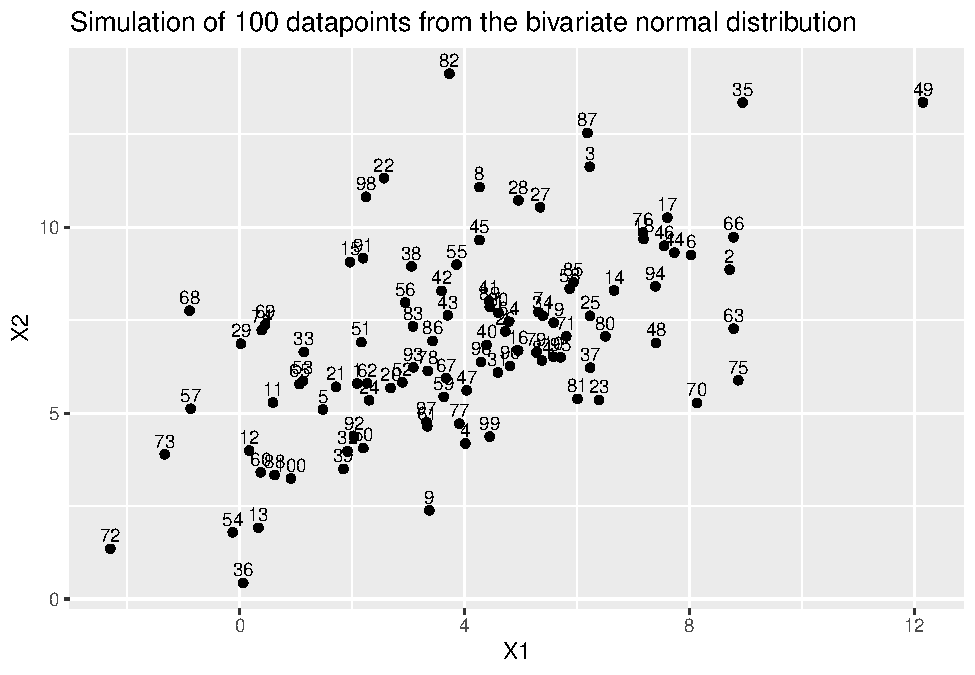
\includegraphics{assignment2_files/figure-latex/unnamed-chunk-2-1.pdf}

\hypertarget{b}{%
\subsection{b)}\label{b}}

Perform the covariance based PCA transformation to the data set.

\begin{Shaded}
\begin{Highlighting}[]
\NormalTok{multinormData.PCA }\OtherTok{\textless{}{-}} \FunctionTok{princomp}\NormalTok{(multinormData,}\AttributeTok{cor=}\ConstantTok{FALSE}\NormalTok{)}

\CommentTok{\# names(multinormData.PCA)}

\FunctionTok{cat}\NormalTok{(}\StringTok{"sdev}\SpecialCharTok{\textbackslash{}n}\StringTok{"}\NormalTok{)}
\end{Highlighting}
\end{Shaded}

\begin{verbatim}
## sdev
\end{verbatim}

\begin{Shaded}
\begin{Highlighting}[]
\NormalTok{multinormData.PCA}\SpecialCharTok{$}\NormalTok{sdev}
\end{Highlighting}
\end{Shaded}

\begin{verbatim}
##   Comp.1   Comp.2 
## 3.308146 1.740956
\end{verbatim}

\begin{Shaded}
\begin{Highlighting}[]
\FunctionTok{cat}\NormalTok{(}\StringTok{"}\SpecialCharTok{\textbackslash{}n}\StringTok{The G matrix (columns are eigenvectors)"}\NormalTok{)}
\end{Highlighting}
\end{Shaded}

\begin{verbatim}
## 
## The G matrix (columns are eigenvectors)
\end{verbatim}

\begin{Shaded}
\begin{Highlighting}[]
\NormalTok{multinormData.PCA}\SpecialCharTok{$}\NormalTok{loadings}
\end{Highlighting}
\end{Shaded}

\begin{verbatim}
## 
## Loadings:
##    Comp.1 Comp.2
## X1  0.730  0.683
## X2  0.683 -0.730
## 
##                Comp.1 Comp.2
## SS loadings       1.0    1.0
## Proportion Var    0.5    0.5
## Cumulative Var    0.5    1.0
\end{verbatim}

\begin{Shaded}
\begin{Highlighting}[]
\FunctionTok{cat}\NormalTok{(}\StringTok{"}\SpecialCharTok{\textbackslash{}n}\StringTok{The Y matrix}\SpecialCharTok{\textbackslash{}n}\StringTok{"}\NormalTok{)}
\end{Highlighting}
\end{Shaded}

\begin{verbatim}
## 
## The Y matrix
\end{verbatim}

\begin{Shaded}
\begin{Highlighting}[]
\NormalTok{multinormData.PCA}\SpecialCharTok{$}\NormalTok{scores}
\end{Highlighting}
\end{Shaded}

\begin{verbatim}
##             Comp.1      Comp.2
##   [1,] -2.17827246 -0.46221980
##   [2,]  4.75262497  1.82729277
##   [3,]  4.82730975 -1.89483414
##   [4,] -1.87109223  2.03210706
##   [5,] -3.09951296 -0.36586466
##   [6,]  4.52410022  1.06874460
##   [7,]  1.49123853  0.33524180
##   [8,]  3.02122043 -2.83432943
##   [9,] -3.56750067  2.90523250
##  [10,]  0.86452524  1.39810492
##  [11,] -3.62112631 -1.10959379
##  [12,] -4.81319762 -0.45511335
##  [13,] -6.11064265  1.17427376
##  [14,]  2.87085593  0.83015426
##  [15,] -0.04140454 -2.93237148
##  [16,]  0.52268395  0.84562948
##  [17,]  4.90085754  0.04729255
##  [18,]  4.19996010  0.17892353
##  [19,]  1.49249564  0.72978018
##  [20,] -1.82513211  0.03249809
##  [21,] -2.51108335 -0.65593438
##  [22,]  1.94167798 -4.16997989
##  [23,]  0.66460325  2.79680870
##  [24,] -2.32834747  0.01317426
##  [25,]  2.09416553  1.03710195
##  [26,]  0.70481207  0.31540707
##  [27,]  3.43629048 -1.70119071
##  [28,]  3.28500283 -2.10370292
##  [29,] -2.95509685 -2.65577047
##  [30,]  0.95721105 -0.13433844
##  [31,] -0.14623075  1.03153253
##  [32,] -3.54489210  0.75074988
##  [33,] -2.29184702 -1.72932982
##  [34,]  1.48078864  0.46242341
##  [35,]  7.99286146 -1.30042475
##  [36,] -7.32165972  2.07528696
##  [37,]  1.14116684  2.05656183
##  [38,]  0.67973242 -2.10170256
##  [39,] -3.92387042  1.04947859
##  [40,]  0.21185361  0.35564027
##  [41,]  1.04944810 -0.48130137
##  [42,]  0.62180026 -1.25638523
##  [43,]  0.25447297 -0.70051348
##  [44,]  4.34813784  0.82114233
##  [45,]  2.04868382 -1.79523985
##  [46,]  4.33895340  0.55875050
##  [47,] -0.87855189  1.00377597
##  [48,]  2.45255079  2.37093962
##  [49,] 10.33837913  0.88795977
##  [50,] -3.28173211  0.88165260
##  [51,] -1.36167924 -1.22346275
##  [52,] -1.56824563  0.06762844
##  [53,] -2.83880849 -1.16849400
##  [54,] -6.52696056  0.95271376
##  [55,]  1.30006233 -1.59206270
##  [56,] -0.06658641 -1.46883587
##  [57,] -4.80189025 -1.98733456
##  [58,]  2.32567267  0.25871621
##  [59,] -1.29808735  0.85285978
##  [60,] -5.05998178  0.11289337
##  [61,] -2.05201952  1.22943550
##  [62,] -2.04173537 -0.34443680
##  [63,]  3.72373950  3.03474839
##  [64,]  0.92654191  0.16747559
##  [65,] -2.93612569 -1.15028626
##  [66,]  5.40046793  1.23571999
##  [67,] -0.92431835  0.51521694
##  [68,] -3.01538270 -3.92971589
##  [69,] -2.29969344 -2.72895597
##  [70,]  1.87719531  4.04974630
##  [71,]  1.40721612  1.15037616
##  [72,] -8.42040845 -0.21017026
##  [73,] -5.97652244 -1.40656950
##  [74,] -2.43670809 -2.66901014
##  [75,]  2.83551004  4.10313157
##  [76,]  4.30833993  0.04191688
##  [77,] -1.58515486  1.56892020
##  [78,] -1.02588149  0.14721945
##  [79,]  0.72047797  1.10717030
##  [80,]  1.91790458  1.62619918
##  [81,]  0.40356508  2.51595575
##  [82,]  4.71328101 -5.42729074
##  [83,] -0.40240209 -0.90595789
##  [84,]  0.64801884  1.33022979
##  [85,]  2.49262247  0.17560007
##  [86,] -0.41584453 -0.37998659
##  [87,]  5.41547621 -2.58597297
##  [88,] -4.92986497  0.33282071
##  [89,]  0.95018939 -0.35316740
##  [90,]  0.13207819  1.05068239
##  [91,]  0.20006836 -2.85008072
##  [92,] -3.19914110  0.54979377
##  [93,] -1.15139083 -0.09664384
##  [94,]  3.48514177  1.25059196
##  [95,]  0.94951798  1.49509384
##  [96,] -0.16953020  0.61601742
##  [97,] -1.98505480  1.13922854
##  [98,]  1.36818432 -4.02416677
##  [99,] -1.42943533  2.19026170
## [100,] -4.78168954  0.60071646
\end{verbatim}

\begin{Shaded}
\begin{Highlighting}[]
\FunctionTok{cat}\NormalTok{(}\StringTok{"}\SpecialCharTok{\textbackslash{}n}\StringTok{The sample mean}\SpecialCharTok{\textbackslash{}n}\StringTok{"}\NormalTok{)}
\end{Highlighting}
\end{Shaded}

\begin{verbatim}
## 
## The sample mean
\end{verbatim}

\begin{Shaded}
\begin{Highlighting}[]
\NormalTok{multinormData.PCA}\SpecialCharTok{$}\NormalTok{center}
\end{Highlighting}
\end{Shaded}

\begin{verbatim}
##       X1       X2 
## 3.992649 6.946177
\end{verbatim}

\begin{Shaded}
\begin{Highlighting}[]
\FunctionTok{cat}\NormalTok{(}\StringTok{"}\SpecialCharTok{\textbackslash{}n}\StringTok{Relevant when cor=TRUE}\SpecialCharTok{\textbackslash{}n}\StringTok{"}\NormalTok{)}
\end{Highlighting}
\end{Shaded}

\begin{verbatim}
## 
## Relevant when cor=TRUE
\end{verbatim}

\begin{Shaded}
\begin{Highlighting}[]
\NormalTok{multinormData.PCA}\SpecialCharTok{$}\NormalTok{scale}
\end{Highlighting}
\end{Shaded}

\begin{verbatim}
## X1 X2 
##  1  1
\end{verbatim}

\begin{Shaded}
\begin{Highlighting}[]
\FunctionTok{cat}\NormalTok{(}\StringTok{"}\SpecialCharTok{\textbackslash{}n}\StringTok{number of observations}\SpecialCharTok{\textbackslash{}n}\StringTok{"}\NormalTok{)}
\end{Highlighting}
\end{Shaded}

\begin{verbatim}
## 
## number of observations
\end{verbatim}

\begin{Shaded}
\begin{Highlighting}[]
\NormalTok{multinormData.PCA}\SpecialCharTok{$}\NormalTok{n.obs}
\end{Highlighting}
\end{Shaded}

\begin{verbatim}
## [1] 100
\end{verbatim}

\begin{Shaded}
\begin{Highlighting}[]
\FunctionTok{cat}\NormalTok{(}\StringTok{"}\SpecialCharTok{\textbackslash{}n}\StringTok{function input}\SpecialCharTok{\textbackslash{}n}\StringTok{"}\NormalTok{)}
\end{Highlighting}
\end{Shaded}

\begin{verbatim}
## 
## function input
\end{verbatim}

\begin{Shaded}
\begin{Highlighting}[]
\NormalTok{multinormData.PCA}\SpecialCharTok{$}\NormalTok{calls}
\end{Highlighting}
\end{Shaded}

\begin{verbatim}
## NULL
\end{verbatim}

\hypertarget{c}{%
\subsection{c)}\label{c}}

Plot the score matrix. Use the same scale as in a) and label the data
points with the corresponding observation number. Choose your scale
(limits for the x- and y-axis) in a way that all the observations are
visible in the figure.\\

\begin{Shaded}
\begin{Highlighting}[]
\FunctionTok{library}\NormalTok{(ggplot2)}
\FunctionTok{ggplot}\NormalTok{(}\FunctionTok{data.frame}\NormalTok{(multinormData.PCA}\SpecialCharTok{$}\NormalTok{scores), }\FunctionTok{aes}\NormalTok{(}\AttributeTok{x =}\NormalTok{ Comp}\FloatTok{.1}\NormalTok{, }\AttributeTok{y =}\NormalTok{ Comp}\FloatTok{.2}\NormalTok{)) }\SpecialCharTok{+} 
  \FunctionTok{geom\_point}\NormalTok{() }\SpecialCharTok{+} \FunctionTok{geom\_text}\NormalTok{(}\AttributeTok{hjust=} \FloatTok{0.5}\NormalTok{, }\AttributeTok{vjust=}\SpecialCharTok{{-}}\FloatTok{0.5}\NormalTok{, }\AttributeTok{label =} \DecValTok{1}\SpecialCharTok{:}\DecValTok{100}\NormalTok{, }\AttributeTok{size=}\DecValTok{3}\NormalTok{) }\SpecialCharTok{+}
  \FunctionTok{ggtitle}\NormalTok{(}\StringTok{"Principle components graph"}\NormalTok{) }\SpecialCharTok{+} 
  \FunctionTok{xlab}\NormalTok{(}\StringTok{"Component 1"}\NormalTok{) }\SpecialCharTok{+} \FunctionTok{ylab}\NormalTok{(}\StringTok{"Component 2"}\NormalTok{) }
\end{Highlighting}
\end{Shaded}

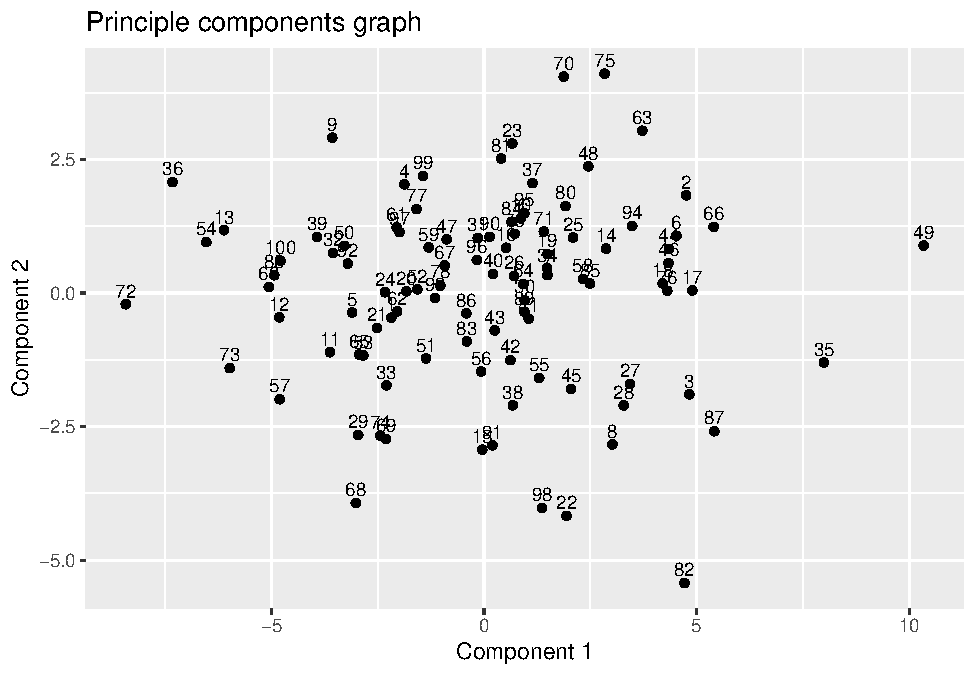
\includegraphics{assignment2_files/figure-latex/unnamed-chunk-4-1.pdf}

\hypertarget{d}{%
\subsection{d)}\label{d}}

Compare the plots of a) and c) and describe the differences.\\

\begin{Shaded}
\begin{Highlighting}[]
\CommentTok{\# Plot data and label points with observation number}
\FunctionTok{ggplot}\NormalTok{(multinormData, }\FunctionTok{aes}\NormalTok{(}\AttributeTok{x =}\NormalTok{ X1, }\AttributeTok{y =}\NormalTok{ X2)) }\SpecialCharTok{+} 
  \FunctionTok{geom\_point}\NormalTok{() }\SpecialCharTok{+} \FunctionTok{geom\_text}\NormalTok{(}\AttributeTok{hjust=} \FloatTok{0.5}\NormalTok{, }\AttributeTok{vjust=}\SpecialCharTok{{-}}\FloatTok{0.5}\NormalTok{, }\AttributeTok{label =} \DecValTok{1}\SpecialCharTok{:}\DecValTok{100}\NormalTok{, }\AttributeTok{size=}\DecValTok{3}\NormalTok{) }\SpecialCharTok{+}
  \FunctionTok{ggtitle}\NormalTok{(}\StringTok{"Simulation of 100 datapoints from the bivariate normal distribution"}\NormalTok{) }\SpecialCharTok{+} 
  \FunctionTok{xlab}\NormalTok{(}\StringTok{"X1"}\NormalTok{) }\SpecialCharTok{+} \FunctionTok{ylab}\NormalTok{(}\StringTok{"X2"}\NormalTok{) }
\end{Highlighting}
\end{Shaded}

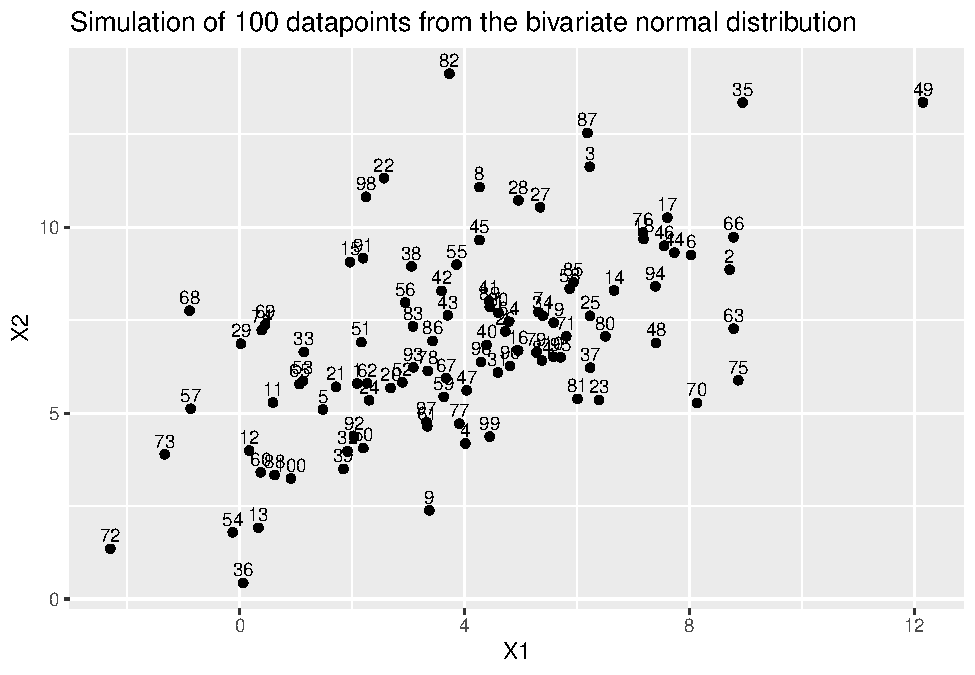
\includegraphics{assignment2_files/figure-latex/unnamed-chunk-5-1.pdf}

\begin{Shaded}
\begin{Highlighting}[]
\FunctionTok{ggplot}\NormalTok{(}\FunctionTok{data.frame}\NormalTok{(multinormData.PCA}\SpecialCharTok{$}\NormalTok{scores), }\FunctionTok{aes}\NormalTok{(}\AttributeTok{x =}\NormalTok{ Comp}\FloatTok{.1}\NormalTok{, }\AttributeTok{y =}\NormalTok{ Comp}\FloatTok{.2}\NormalTok{)) }\SpecialCharTok{+} 
  \FunctionTok{geom\_point}\NormalTok{() }\SpecialCharTok{+} \FunctionTok{geom\_text}\NormalTok{(}\AttributeTok{hjust=} \FloatTok{0.5}\NormalTok{, }\AttributeTok{vjust=}\SpecialCharTok{{-}}\FloatTok{0.5}\NormalTok{, }\AttributeTok{label =} \DecValTok{1}\SpecialCharTok{:}\DecValTok{100}\NormalTok{, }\AttributeTok{size=}\DecValTok{3}\NormalTok{) }\SpecialCharTok{+}
  \FunctionTok{ggtitle}\NormalTok{(}\StringTok{"Principal components graph"}\NormalTok{) }\SpecialCharTok{+} 
  \FunctionTok{xlab}\NormalTok{(}\StringTok{"Component 1"}\NormalTok{) }\SpecialCharTok{+} \FunctionTok{ylab}\NormalTok{(}\StringTok{"Component 2"}\NormalTok{) }
\end{Highlighting}
\end{Shaded}

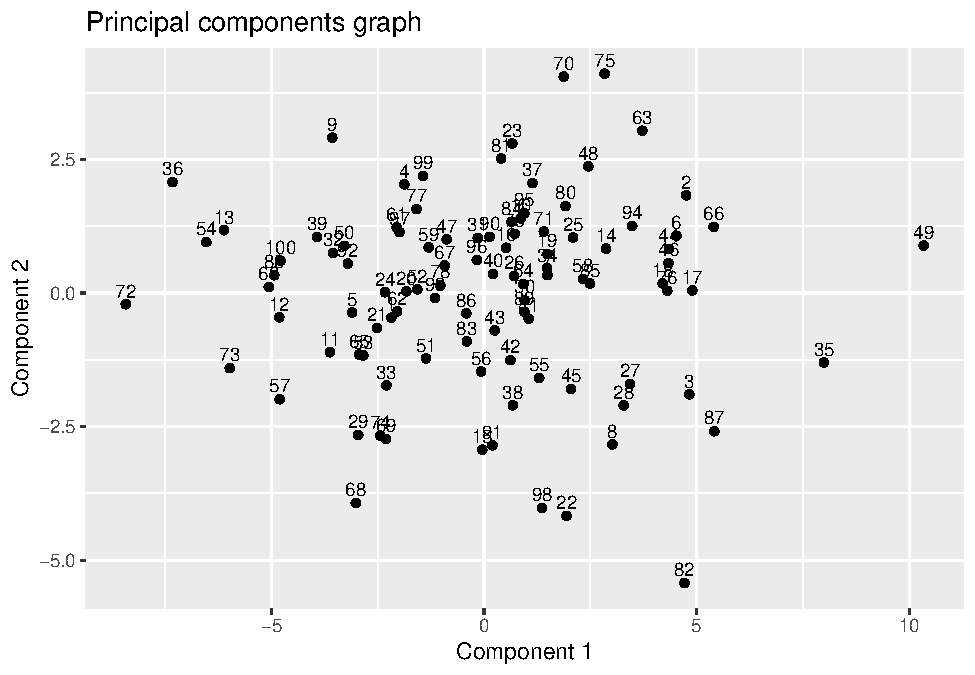
\includegraphics{assignment2_files/figure-latex/unnamed-chunk-5-2.pdf}
We can observe that the PCA transform has rotated the original data to
be orthogonal to the axis. This is because the principal components are
the eigenvectors of the covariance matrix of the data, which tries to
maximize the difference between the datapoints. The first component has
the largest eigenvalue, the second component has the second largest
eigenvalue and so on. So in short, the difference between them is that
the covariance between the original data is nonzero, while the
covariance under the PCA transformed graph is zero or nearly zero.\\

\hypertarget{e}{%
\subsection{e)}\label{e}}

Calculate the \(G\) and \(Y\) matrices without using any existing PCA
functions. Note that the function princomp scales the covariance matrix
with \(1/n\) (instead of the usual \(1/(n-1)\)). Attach the R code to
your solution.\\

The matrix G is the eigenvector matrix of the sample covariance matrix
\(\Sigma\) The matrix Y is the sample PCA transformation:
\(Y = (X - 1_n\overline{x}^T)G\)

Model reference

\begin{Shaded}
\begin{Highlighting}[]
\FunctionTok{cat}\NormalTok{(}\StringTok{"}\SpecialCharTok{\textbackslash{}n}\StringTok{The G matrix (columns are eigenvectors)"}\NormalTok{)}
\end{Highlighting}
\end{Shaded}

\begin{verbatim}
## 
## The G matrix (columns are eigenvectors)
\end{verbatim}

\begin{Shaded}
\begin{Highlighting}[]
\NormalTok{multinormData.PCA}\SpecialCharTok{$}\NormalTok{loadings}
\end{Highlighting}
\end{Shaded}

\begin{verbatim}
## 
## Loadings:
##    Comp.1 Comp.2
## X1  0.730  0.683
## X2  0.683 -0.730
## 
##                Comp.1 Comp.2
## SS loadings       1.0    1.0
## Proportion Var    0.5    0.5
## Cumulative Var    0.5    1.0
\end{verbatim}

\begin{Shaded}
\begin{Highlighting}[]
\FunctionTok{cat}\NormalTok{(}\StringTok{"}\SpecialCharTok{\textbackslash{}n}\StringTok{The Y matrix}\SpecialCharTok{\textbackslash{}n}\StringTok{"}\NormalTok{)}
\end{Highlighting}
\end{Shaded}

\begin{verbatim}
## 
## The Y matrix
\end{verbatim}

\begin{Shaded}
\begin{Highlighting}[]
\NormalTok{multinormData.PCA}\SpecialCharTok{$}\NormalTok{scores}
\end{Highlighting}
\end{Shaded}

\begin{verbatim}
##             Comp.1      Comp.2
##   [1,] -2.17827246 -0.46221980
##   [2,]  4.75262497  1.82729277
##   [3,]  4.82730975 -1.89483414
##   [4,] -1.87109223  2.03210706
##   [5,] -3.09951296 -0.36586466
##   [6,]  4.52410022  1.06874460
##   [7,]  1.49123853  0.33524180
##   [8,]  3.02122043 -2.83432943
##   [9,] -3.56750067  2.90523250
##  [10,]  0.86452524  1.39810492
##  [11,] -3.62112631 -1.10959379
##  [12,] -4.81319762 -0.45511335
##  [13,] -6.11064265  1.17427376
##  [14,]  2.87085593  0.83015426
##  [15,] -0.04140454 -2.93237148
##  [16,]  0.52268395  0.84562948
##  [17,]  4.90085754  0.04729255
##  [18,]  4.19996010  0.17892353
##  [19,]  1.49249564  0.72978018
##  [20,] -1.82513211  0.03249809
##  [21,] -2.51108335 -0.65593438
##  [22,]  1.94167798 -4.16997989
##  [23,]  0.66460325  2.79680870
##  [24,] -2.32834747  0.01317426
##  [25,]  2.09416553  1.03710195
##  [26,]  0.70481207  0.31540707
##  [27,]  3.43629048 -1.70119071
##  [28,]  3.28500283 -2.10370292
##  [29,] -2.95509685 -2.65577047
##  [30,]  0.95721105 -0.13433844
##  [31,] -0.14623075  1.03153253
##  [32,] -3.54489210  0.75074988
##  [33,] -2.29184702 -1.72932982
##  [34,]  1.48078864  0.46242341
##  [35,]  7.99286146 -1.30042475
##  [36,] -7.32165972  2.07528696
##  [37,]  1.14116684  2.05656183
##  [38,]  0.67973242 -2.10170256
##  [39,] -3.92387042  1.04947859
##  [40,]  0.21185361  0.35564027
##  [41,]  1.04944810 -0.48130137
##  [42,]  0.62180026 -1.25638523
##  [43,]  0.25447297 -0.70051348
##  [44,]  4.34813784  0.82114233
##  [45,]  2.04868382 -1.79523985
##  [46,]  4.33895340  0.55875050
##  [47,] -0.87855189  1.00377597
##  [48,]  2.45255079  2.37093962
##  [49,] 10.33837913  0.88795977
##  [50,] -3.28173211  0.88165260
##  [51,] -1.36167924 -1.22346275
##  [52,] -1.56824563  0.06762844
##  [53,] -2.83880849 -1.16849400
##  [54,] -6.52696056  0.95271376
##  [55,]  1.30006233 -1.59206270
##  [56,] -0.06658641 -1.46883587
##  [57,] -4.80189025 -1.98733456
##  [58,]  2.32567267  0.25871621
##  [59,] -1.29808735  0.85285978
##  [60,] -5.05998178  0.11289337
##  [61,] -2.05201952  1.22943550
##  [62,] -2.04173537 -0.34443680
##  [63,]  3.72373950  3.03474839
##  [64,]  0.92654191  0.16747559
##  [65,] -2.93612569 -1.15028626
##  [66,]  5.40046793  1.23571999
##  [67,] -0.92431835  0.51521694
##  [68,] -3.01538270 -3.92971589
##  [69,] -2.29969344 -2.72895597
##  [70,]  1.87719531  4.04974630
##  [71,]  1.40721612  1.15037616
##  [72,] -8.42040845 -0.21017026
##  [73,] -5.97652244 -1.40656950
##  [74,] -2.43670809 -2.66901014
##  [75,]  2.83551004  4.10313157
##  [76,]  4.30833993  0.04191688
##  [77,] -1.58515486  1.56892020
##  [78,] -1.02588149  0.14721945
##  [79,]  0.72047797  1.10717030
##  [80,]  1.91790458  1.62619918
##  [81,]  0.40356508  2.51595575
##  [82,]  4.71328101 -5.42729074
##  [83,] -0.40240209 -0.90595789
##  [84,]  0.64801884  1.33022979
##  [85,]  2.49262247  0.17560007
##  [86,] -0.41584453 -0.37998659
##  [87,]  5.41547621 -2.58597297
##  [88,] -4.92986497  0.33282071
##  [89,]  0.95018939 -0.35316740
##  [90,]  0.13207819  1.05068239
##  [91,]  0.20006836 -2.85008072
##  [92,] -3.19914110  0.54979377
##  [93,] -1.15139083 -0.09664384
##  [94,]  3.48514177  1.25059196
##  [95,]  0.94951798  1.49509384
##  [96,] -0.16953020  0.61601742
##  [97,] -1.98505480  1.13922854
##  [98,]  1.36818432 -4.02416677
##  [99,] -1.42943533  2.19026170
## [100,] -4.78168954  0.60071646
\end{verbatim}

\begin{Shaded}
\begin{Highlighting}[]
\NormalTok{calculateG }\OtherTok{\textless{}{-}} \ControlFlowTok{function}\NormalTok{(multinormData)\{}
\NormalTok{  covarianceMatrix }\OtherTok{\textless{}{-}} \FunctionTok{cov}\NormalTok{(multinormData)}
\NormalTok{  G }\OtherTok{\textless{}{-}} \FunctionTok{eigen}\NormalTok{(covarianceMatrix)}\SpecialCharTok{$}\NormalTok{vectors}
  \FunctionTok{return}\NormalTok{(G)}
\NormalTok{\}}

\NormalTok{calculateY }\OtherTok{\textless{}{-}} \ControlFlowTok{function}\NormalTok{(multinormData, G)\{}
\NormalTok{  n }\OtherTok{\textless{}{-}} \FunctionTok{nrow}\NormalTok{(multinormData)}
\NormalTok{  meanData }\OtherTok{\textless{}{-}} \FunctionTok{colMeans}\NormalTok{(multinormData)}
\NormalTok{  centered }\OtherTok{\textless{}{-}} \FunctionTok{sweep}\NormalTok{(multinormData, }\DecValTok{2}\NormalTok{, meanData, }\StringTok{"{-}"}\NormalTok{)}
\NormalTok{  Y }\OtherTok{\textless{}{-}} \FunctionTok{as.matrix}\NormalTok{(centered) }\SpecialCharTok{\%*\%}\NormalTok{ (G) }
  \FunctionTok{return}\NormalTok{(Y)}
\NormalTok{\}}

\NormalTok{G }\OtherTok{\textless{}{-}} \FunctionTok{calculateG}\NormalTok{(multinormData)}
\FunctionTok{cat}\NormalTok{(}\StringTok{"The matrix G is}\SpecialCharTok{\textbackslash{}n}\StringTok{"}\NormalTok{)}
\end{Highlighting}
\end{Shaded}

\begin{verbatim}
## The matrix G is
\end{verbatim}

\begin{Shaded}
\begin{Highlighting}[]
\FunctionTok{print}\NormalTok{(G)}
\end{Highlighting}
\end{Shaded}

\begin{verbatim}
##            [,1]       [,2]
## [1,] -0.7304868  0.6829268
## [2,] -0.6829268 -0.7304868
\end{verbatim}

\begin{Shaded}
\begin{Highlighting}[]
\NormalTok{Y }\OtherTok{\textless{}{-}} \FunctionTok{calculateY}\NormalTok{(multinormData, G)}
\FunctionTok{cat}\NormalTok{(}\StringTok{"}\SpecialCharTok{\textbackslash{}n}\StringTok{The matrix Y is}\SpecialCharTok{\textbackslash{}n}\StringTok{"}\NormalTok{)}
\end{Highlighting}
\end{Shaded}

\begin{verbatim}
## 
## The matrix Y is
\end{verbatim}

\begin{Shaded}
\begin{Highlighting}[]
\FunctionTok{print}\NormalTok{(Y)}
\end{Highlighting}
\end{Shaded}

\begin{verbatim}
##                [,1]        [,2]
##   [1,]   2.17827246 -0.46221980
##   [2,]  -4.75262497  1.82729277
##   [3,]  -4.82730975 -1.89483414
##   [4,]   1.87109223  2.03210706
##   [5,]   3.09951296 -0.36586466
##   [6,]  -4.52410022  1.06874460
##   [7,]  -1.49123853  0.33524180
##   [8,]  -3.02122043 -2.83432943
##   [9,]   3.56750067  2.90523250
##  [10,]  -0.86452524  1.39810492
##  [11,]   3.62112631 -1.10959379
##  [12,]   4.81319762 -0.45511335
##  [13,]   6.11064265  1.17427376
##  [14,]  -2.87085593  0.83015426
##  [15,]   0.04140454 -2.93237148
##  [16,]  -0.52268395  0.84562948
##  [17,]  -4.90085754  0.04729255
##  [18,]  -4.19996010  0.17892353
##  [19,]  -1.49249564  0.72978018
##  [20,]   1.82513211  0.03249809
##  [21,]   2.51108335 -0.65593438
##  [22,]  -1.94167798 -4.16997989
##  [23,]  -0.66460325  2.79680870
##  [24,]   2.32834747  0.01317426
##  [25,]  -2.09416553  1.03710195
##  [26,]  -0.70481207  0.31540707
##  [27,]  -3.43629048 -1.70119071
##  [28,]  -3.28500283 -2.10370292
##  [29,]   2.95509685 -2.65577047
##  [30,]  -0.95721105 -0.13433844
##  [31,]   0.14623075  1.03153253
##  [32,]   3.54489210  0.75074988
##  [33,]   2.29184702 -1.72932982
##  [34,]  -1.48078864  0.46242341
##  [35,]  -7.99286146 -1.30042475
##  [36,]   7.32165972  2.07528696
##  [37,]  -1.14116684  2.05656183
##  [38,]  -0.67973242 -2.10170256
##  [39,]   3.92387042  1.04947859
##  [40,]  -0.21185361  0.35564027
##  [41,]  -1.04944810 -0.48130137
##  [42,]  -0.62180026 -1.25638523
##  [43,]  -0.25447297 -0.70051348
##  [44,]  -4.34813784  0.82114233
##  [45,]  -2.04868382 -1.79523985
##  [46,]  -4.33895340  0.55875050
##  [47,]   0.87855189  1.00377597
##  [48,]  -2.45255079  2.37093962
##  [49,] -10.33837913  0.88795977
##  [50,]   3.28173211  0.88165260
##  [51,]   1.36167924 -1.22346275
##  [52,]   1.56824563  0.06762844
##  [53,]   2.83880849 -1.16849400
##  [54,]   6.52696056  0.95271376
##  [55,]  -1.30006233 -1.59206270
##  [56,]   0.06658641 -1.46883587
##  [57,]   4.80189025 -1.98733456
##  [58,]  -2.32567267  0.25871621
##  [59,]   1.29808735  0.85285978
##  [60,]   5.05998178  0.11289337
##  [61,]   2.05201952  1.22943550
##  [62,]   2.04173537 -0.34443680
##  [63,]  -3.72373950  3.03474839
##  [64,]  -0.92654191  0.16747559
##  [65,]   2.93612569 -1.15028626
##  [66,]  -5.40046793  1.23571999
##  [67,]   0.92431835  0.51521694
##  [68,]   3.01538270 -3.92971589
##  [69,]   2.29969344 -2.72895597
##  [70,]  -1.87719531  4.04974630
##  [71,]  -1.40721612  1.15037616
##  [72,]   8.42040845 -0.21017026
##  [73,]   5.97652244 -1.40656950
##  [74,]   2.43670809 -2.66901014
##  [75,]  -2.83551004  4.10313157
##  [76,]  -4.30833993  0.04191688
##  [77,]   1.58515486  1.56892020
##  [78,]   1.02588149  0.14721945
##  [79,]  -0.72047797  1.10717030
##  [80,]  -1.91790458  1.62619918
##  [81,]  -0.40356508  2.51595575
##  [82,]  -4.71328101 -5.42729074
##  [83,]   0.40240209 -0.90595789
##  [84,]  -0.64801884  1.33022979
##  [85,]  -2.49262247  0.17560007
##  [86,]   0.41584453 -0.37998659
##  [87,]  -5.41547621 -2.58597297
##  [88,]   4.92986497  0.33282071
##  [89,]  -0.95018939 -0.35316740
##  [90,]  -0.13207819  1.05068239
##  [91,]  -0.20006836 -2.85008072
##  [92,]   3.19914110  0.54979377
##  [93,]   1.15139083 -0.09664384
##  [94,]  -3.48514177  1.25059196
##  [95,]  -0.94951798  1.49509384
##  [96,]   0.16953020  0.61601742
##  [97,]   1.98505480  1.13922854
##  [98,]  -1.36818432 -4.02416677
##  [99,]   1.42943533  2.19026170
## [100,]   4.78168954  0.60071646
\end{verbatim}

Note that the sign of the eigenvectors does not matter. Therefore, the
matrix G produced here matches the referenced G matrix above by putting
minus sign on the first component

\hypertarget{f}{%
\subsection{f)}\label{f}}

Verify that the estimated scores and the loadings are equal (up to
signs) in parts b) and e). Hint: If parts b) and e) are done correctly,
the scores and loadings should be the same up to heterogeneous sign
changes.

Yes, they are equal, please scroll up to check part (b) and (e) again.
The matrix G is the loadings matrix and the matrix Y is the scores
matrix. Together, they make up the PCA transformation matrix, where the
G * Y = PCA.

\hypertarget{g}{%
\subsection{g)}\label{g}}

Plot the directions of the first and second principal component to the
original data. The function arrows might be useful.

\begin{Shaded}
\begin{Highlighting}[]
\NormalTok{x }\OtherTok{\textless{}{-}}\NormalTok{ multinormData.PCA}\SpecialCharTok{$}\NormalTok{center[}\StringTok{"X1"}\NormalTok{]}
\NormalTok{y }\OtherTok{\textless{}{-}}\NormalTok{ multinormData.PCA}\SpecialCharTok{$}\NormalTok{center[}\StringTok{"X2"}\NormalTok{]}
\NormalTok{eigenVectorComponent1 }\OtherTok{\textless{}{-}} \FunctionTok{loadings}\NormalTok{(multinormData.PCA)[}\DecValTok{1}\SpecialCharTok{:}\DecValTok{2}\NormalTok{, }\DecValTok{1}\NormalTok{]}
\NormalTok{eigenVectorComponent2 }\OtherTok{\textless{}{-}} \FunctionTok{loadings}\NormalTok{(multinormData.PCA)[}\DecValTok{1}\SpecialCharTok{:}\DecValTok{2}\NormalTok{, }\DecValTok{2}\NormalTok{]}

\CommentTok{\# Plot data and label points with observation number}
\FunctionTok{ggplot}\NormalTok{(multinormData, }\FunctionTok{aes}\NormalTok{(}\AttributeTok{x =}\NormalTok{ X1, }\AttributeTok{y =}\NormalTok{ X2)) }\SpecialCharTok{+} 
  \FunctionTok{geom\_point}\NormalTok{() }\SpecialCharTok{+}
  \FunctionTok{ggtitle}\NormalTok{(}\StringTok{"Simulation of 100 datapoints from the bivariate normal distribution"}\NormalTok{) }\SpecialCharTok{+} 
  \FunctionTok{xlab}\NormalTok{(}\StringTok{"X1"}\NormalTok{) }\SpecialCharTok{+} \FunctionTok{ylab}\NormalTok{(}\StringTok{"X2"}\NormalTok{) }\SpecialCharTok{+} 
  \FunctionTok{geom\_segment}\NormalTok{(}\FunctionTok{aes}\NormalTok{(}\AttributeTok{x =}\NormalTok{ x, }\AttributeTok{y =}\NormalTok{ y, }\AttributeTok{xend =}\NormalTok{ x }\SpecialCharTok{+} \DecValTok{2} \SpecialCharTok{*}\NormalTok{ eigenVectorComponent1[}\DecValTok{1}\NormalTok{], }\AttributeTok{yend =}\NormalTok{ y }\SpecialCharTok{+} \DecValTok{2} \SpecialCharTok{*}\NormalTok{ eigenVectorComponent1[}\DecValTok{2}\NormalTok{]),}
                \AttributeTok{arrow =} \FunctionTok{arrow}\NormalTok{(}\AttributeTok{length =} \FunctionTok{unit}\NormalTok{(}\FloatTok{0.2}\NormalTok{, }\StringTok{"cm"}\NormalTok{), }\AttributeTok{type =} \StringTok{"closed"}\NormalTok{),}
                \AttributeTok{color =} \StringTok{"red"}\NormalTok{, }\AttributeTok{size =} \DecValTok{1}\NormalTok{) }\SpecialCharTok{+}
  \FunctionTok{annotate}\NormalTok{(}\StringTok{"text"}\NormalTok{, }\AttributeTok{x =}\NormalTok{ x }\SpecialCharTok{+} \DecValTok{2} \SpecialCharTok{*}\NormalTok{ eigenVectorComponent1[}\DecValTok{1}\NormalTok{] }\SpecialCharTok{+} \DecValTok{1}\NormalTok{, }\AttributeTok{y =}\NormalTok{ y }\SpecialCharTok{+} \DecValTok{2} \SpecialCharTok{*}\NormalTok{ eigenVectorComponent1[}\DecValTok{2}\NormalTok{] }\SpecialCharTok{+} \FloatTok{0.5}\NormalTok{, }\AttributeTok{label =} \StringTok{"First component"}\NormalTok{, }\AttributeTok{color =} \StringTok{"red"}\NormalTok{, }\AttributeTok{size =} \DecValTok{5}\NormalTok{) }\SpecialCharTok{+}   \FunctionTok{geom\_segment}\NormalTok{(}\FunctionTok{aes}\NormalTok{(}\AttributeTok{x =}\NormalTok{ x, }\AttributeTok{y =}\NormalTok{ y, }\AttributeTok{xend =}\NormalTok{ x }\SpecialCharTok{+} \DecValTok{2} \SpecialCharTok{*}\NormalTok{ eigenVectorComponent2[}\DecValTok{1}\NormalTok{], }\AttributeTok{yend =}\NormalTok{ y }\SpecialCharTok{+} \DecValTok{2} \SpecialCharTok{*}\NormalTok{ eigenVectorComponent2[}\DecValTok{2}\NormalTok{]),}
                \AttributeTok{arrow =} \FunctionTok{arrow}\NormalTok{(}\AttributeTok{length =} \FunctionTok{unit}\NormalTok{(}\FloatTok{0.2}\NormalTok{, }\StringTok{"cm"}\NormalTok{), }\AttributeTok{type =} \StringTok{"closed"}\NormalTok{),}
                \AttributeTok{color =} \StringTok{"red"}\NormalTok{, }\AttributeTok{size =} \DecValTok{1}\NormalTok{) }\SpecialCharTok{+}
  \FunctionTok{annotate}\NormalTok{(}\StringTok{"text"}\NormalTok{, }\AttributeTok{x =}\NormalTok{ x }\SpecialCharTok{+} \DecValTok{2} \SpecialCharTok{*}\NormalTok{ eigenVectorComponent2[}\DecValTok{1}\NormalTok{] }\SpecialCharTok{+} \DecValTok{2}\NormalTok{, }\AttributeTok{y =}\NormalTok{ y }\SpecialCharTok{+} \DecValTok{2} \SpecialCharTok{*}\NormalTok{ eigenVectorComponent2[}\DecValTok{2}\NormalTok{] }\SpecialCharTok{{-}} \DecValTok{1}\NormalTok{, }\AttributeTok{label =} \StringTok{"Second component"}\NormalTok{, }\AttributeTok{color =} \StringTok{"red"}\NormalTok{, }\AttributeTok{size =} \DecValTok{5}\NormalTok{)}
\end{Highlighting}
\end{Shaded}

\begin{verbatim}
## Warning: Using `size` aesthetic for lines was deprecated in ggplot2 3.4.0.
## i Please use `linewidth` instead.
\end{verbatim}

\includegraphics{assignment2_files/figure-latex/unnamed-chunk-8-1.pdf}

\end{document}
